\chapter{Serial Entrepreneurs: Obstacles, Time, and Team}

In this School of Hard Knocks interview, curated here in chapter form by LazyingArt LLC, the formal mathematics is light, but the structure is exact. We are given a small operating system for entrepreneurship: first the scale of the portfolio, then the advice for entering the game, then the deepest bottleneck, and finally the mechanism that relaxes that bottleneck. The notes should therefore preserve the order in which the ideas arrive. The speaker does not begin with abstraction. He begins by counting.

\section{Opening Position: Five Companies, Mixed Ownership}

The opening statement is brief, but it does important work. The speaker owns five companies. Of these, three are run on his own, while the remainder involve partners. This is the only explicit arithmetic relation in the lecture, and it gives the rest of the discussion a concrete scale.

\begin{align}
N_{\mathrm{total}} &= 5, &
N_{\mathrm{solo}} &= 3.
\end{align}

The partnered portion is then obtained by subtraction:

\begin{align}
N_{\mathrm{partnered}}
  &= N_{\mathrm{total}} - N_{\mathrm{solo}} \\
  &= 5 - 3 \\
  &= 2.
\end{align}

\paragraph{Worked derivation.}
This little derivation is almost trivial, but it is not dispensable. It tells us that the speaker is not talking about a single isolated venture. We are already in the regime of multiple moving parts, and so the later discussion of time pressure and the importance of partners is not decorative; it is forced by the scale of the system.

One may summarize the opening in a compact bookkeeping identity:
\begin{equation}
\text{portfolio} = \text{solo ventures} + \text{partnered ventures}.
\end{equation}
Nothing deeper is claimed here. The point is simply that the initial numerical split sets the stage for everything that follows.

\section{Advice for Starting in 2023}

The interviewer then pivots outward. Having established that the speaker operates at nontrivial scale, the conversation asks what advice he would give to someone starting a business in the present moment. The first answer is not technical. It is an operating stance: grind.

That word is intentionally compressed. It does not yet tell us what the rule of motion is, but it tells us that the speaker treats entrepreneurship as something that requires sustained effort rather than occasional inspiration. The lecture then sharpens the idea immediately. The point is not only to work hard, but also to refuse the idea that a negative response is final.

\section{Rejection as Search Logic}

Here the lecture becomes more precise. A ``no'' is not taken as an endpoint. It is treated as information that redirects effort. We can write the rule schematically as
\begin{equation}
\text{No} \not\Rightarrow \text{stop},
\qquad
\text{No} \to \text{another path toward Yes}.
\end{equation}

This is not a theorem about probability, and it is not a sales formula. It is a disciplined way of interpreting failure. The speaker's advice is that rejection should update the route, not cancel the aim.

If we want a slightly more explicit schematic, we may introduce a path variable \(P_k\) for the \(k\)-th attempted route toward a fixed goal. Then the advice may be compressed into the update rule
\begin{equation}
P_{k+1} \neq P_k,
\qquad
G(P_{k+1}) = G(P_k),
\end{equation}
where the goal is held fixed while the route is changed. This notation is editorial rather than spoken, but it captures the rhythm of the answer exactly: the destination remains; the path is revised.

What matters here is the sequence. The lecture does not leave us with ``grind'' as empty exhortation. It immediately converts grit into a search rule. We do not stop at the first obstruction. We re-route.

\section{The Central Obstacle}

At this point the interview makes its most important turn. We move from advice for the beginner to the hardest problem in the speaker's own practice. This is the point where the chapter should preserve the tension rather than flatten it into summary.

\subsection{Question \& Answer}

\paragraph{Question.}
What has been the biggest challenge as a business owner, and how has that challenge been overcome?

\paragraph{Answer.}
Time.

The force of the answer lies in its abruptness. After a brief discussion of work and persistence, the speaker names the true bottleneck in a single word. The lecture then explains why time is not merely one difficulty among others. It is the variable that governs exposure. If one steps away even briefly, the state of the business may already have changed.

This is the local conceptual hinge of the chapter. The earlier advice concerns motion through resistance. The answer here concerns the impossibility of maintaining perfect supervision across multiple growing ventures.

\section{Time as the Primary Scarcity}

To express the point compactly, let \(t_{\mathrm{off}}\) denote time away from active attention, measured in hours, and let \(S(t)\) be a shorthand for the state of the business at time \(t\). Then the speaker's claim may be rendered as
\begin{equation}
t_{\mathrm{off}} \in [1,2]\ \text{hours}
\quad \Longrightarrow \quad
S(t)\ \text{may change materially}.
\end{equation}

\begin{remark}
The symbol \(S(t)\) is only a compact editorial device. The lecture does not introduce a formal state variable. It speaks in ordinary language: take an hour or two off, and something can change.
\end{remark}

The content, however, is quite sharp. Time is scarce not because the entrepreneur wishes to be busy, but because a growing business is dynamic. Conditions move while attention is elsewhere. The deeper issue is therefore not simply workload; it is mismatch between the number of evolving commitments and the continuity of a single person's oversight.

This is why the opening arithmetic mattered. Five companies with mixed ownership already imply a structure in which the speaker cannot be everywhere at once. The numerical statement at the beginning and the time statement here belong to the same argument.

\section{Partners, Team, and Continuity of Execution}

Once time is named as the bottleneck, the lecture asks for the mechanism that relaxes it. The answer is not mystical. It is organizational. Partners in the growing businesses have been the most helpful thing. The lesson then broadens one step further: if one has the right team, one can do it.

We may summarize the logic by the causal chain
\begin{equation}
\text{time scarcity}
\to
\text{partners}
\to
\text{right team}
\to
\text{continuity of execution}.
\end{equation}

The movement from partners to team is important. ``Partners'' refers to the speaker's own concrete arrangement. ``Right team'' is the general principle extracted from it. The chapter should preserve this widening of scope.

\begin{figure}
\centering
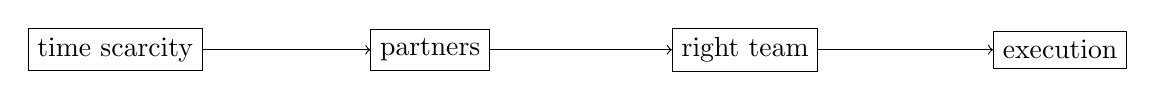
\begin{tikzpicture}
\node[draw, rectangle] (t) at (0,0) {time scarcity};
\node[draw, rectangle] (p) at (4,0) {partners};
\node[draw, rectangle] (r) at (8,0) {right team};
\node[draw, rectangle] (e) at (12,0) {execution};
\draw[->] (t) -- (p);
\draw[->] (p) -- (r);
\draw[->] (r) -- (e);
\end{tikzpicture}
\end{figure}

The figure is only a schematic summary of the verbal logic. Still, it helps us see the structure clearly. The problem is not solved by heroic effort alone. Effort governs persistence, but organization governs continuity. The speaker's sequence is therefore perfectly coherent:

\begin{enumerate}
\item multiple ventures create scale,
\item scale creates a pressure on attention,
\item limited attention makes time the bottleneck,
\item partners distribute that burden,
\item the right team turns local relief into a durable operating principle.
\end{enumerate}

We should resist the temptation to over-formalize this. No staffing law is offered. No theory of delegation efficiency is given. The lecture remains concrete. But even in its brevity, it presents a genuine mechanism: one person cannot absorb all change across a growing portfolio, and so the problem must be solved structurally rather than emotionally.

\section{Summary}

The chapter is short because the interview is short, but the progression is clean. We begin with a count:
\[
5 = 3 + 2,
\]
meaning five companies in all, three operated independently and two with partners. From that factual base the lecture gives advice for the beginner: work hard, and do not interpret rejection as termination. Then it poses the central practical question: what is the hardest part of ownership? The answer is time. A brief absence can matter. That is why partners help, and why the right team becomes the general law.

The final lesson is therefore not merely motivational. Persistence matters, but it is not enough. When scale outruns individual attention, the durable answer is organizational leverage. That is the chapter's real payoff.